\chapter{Kanban Setup \\
\small{\textit{-- Matthew Smith, Bowen Jiang, Gleb Myshkin}}
\label{Chapter::Kanban Setup1}}
\index{Chapter!Kanban Setup}
\index{Kanban Board}

\begin{figure} [H]
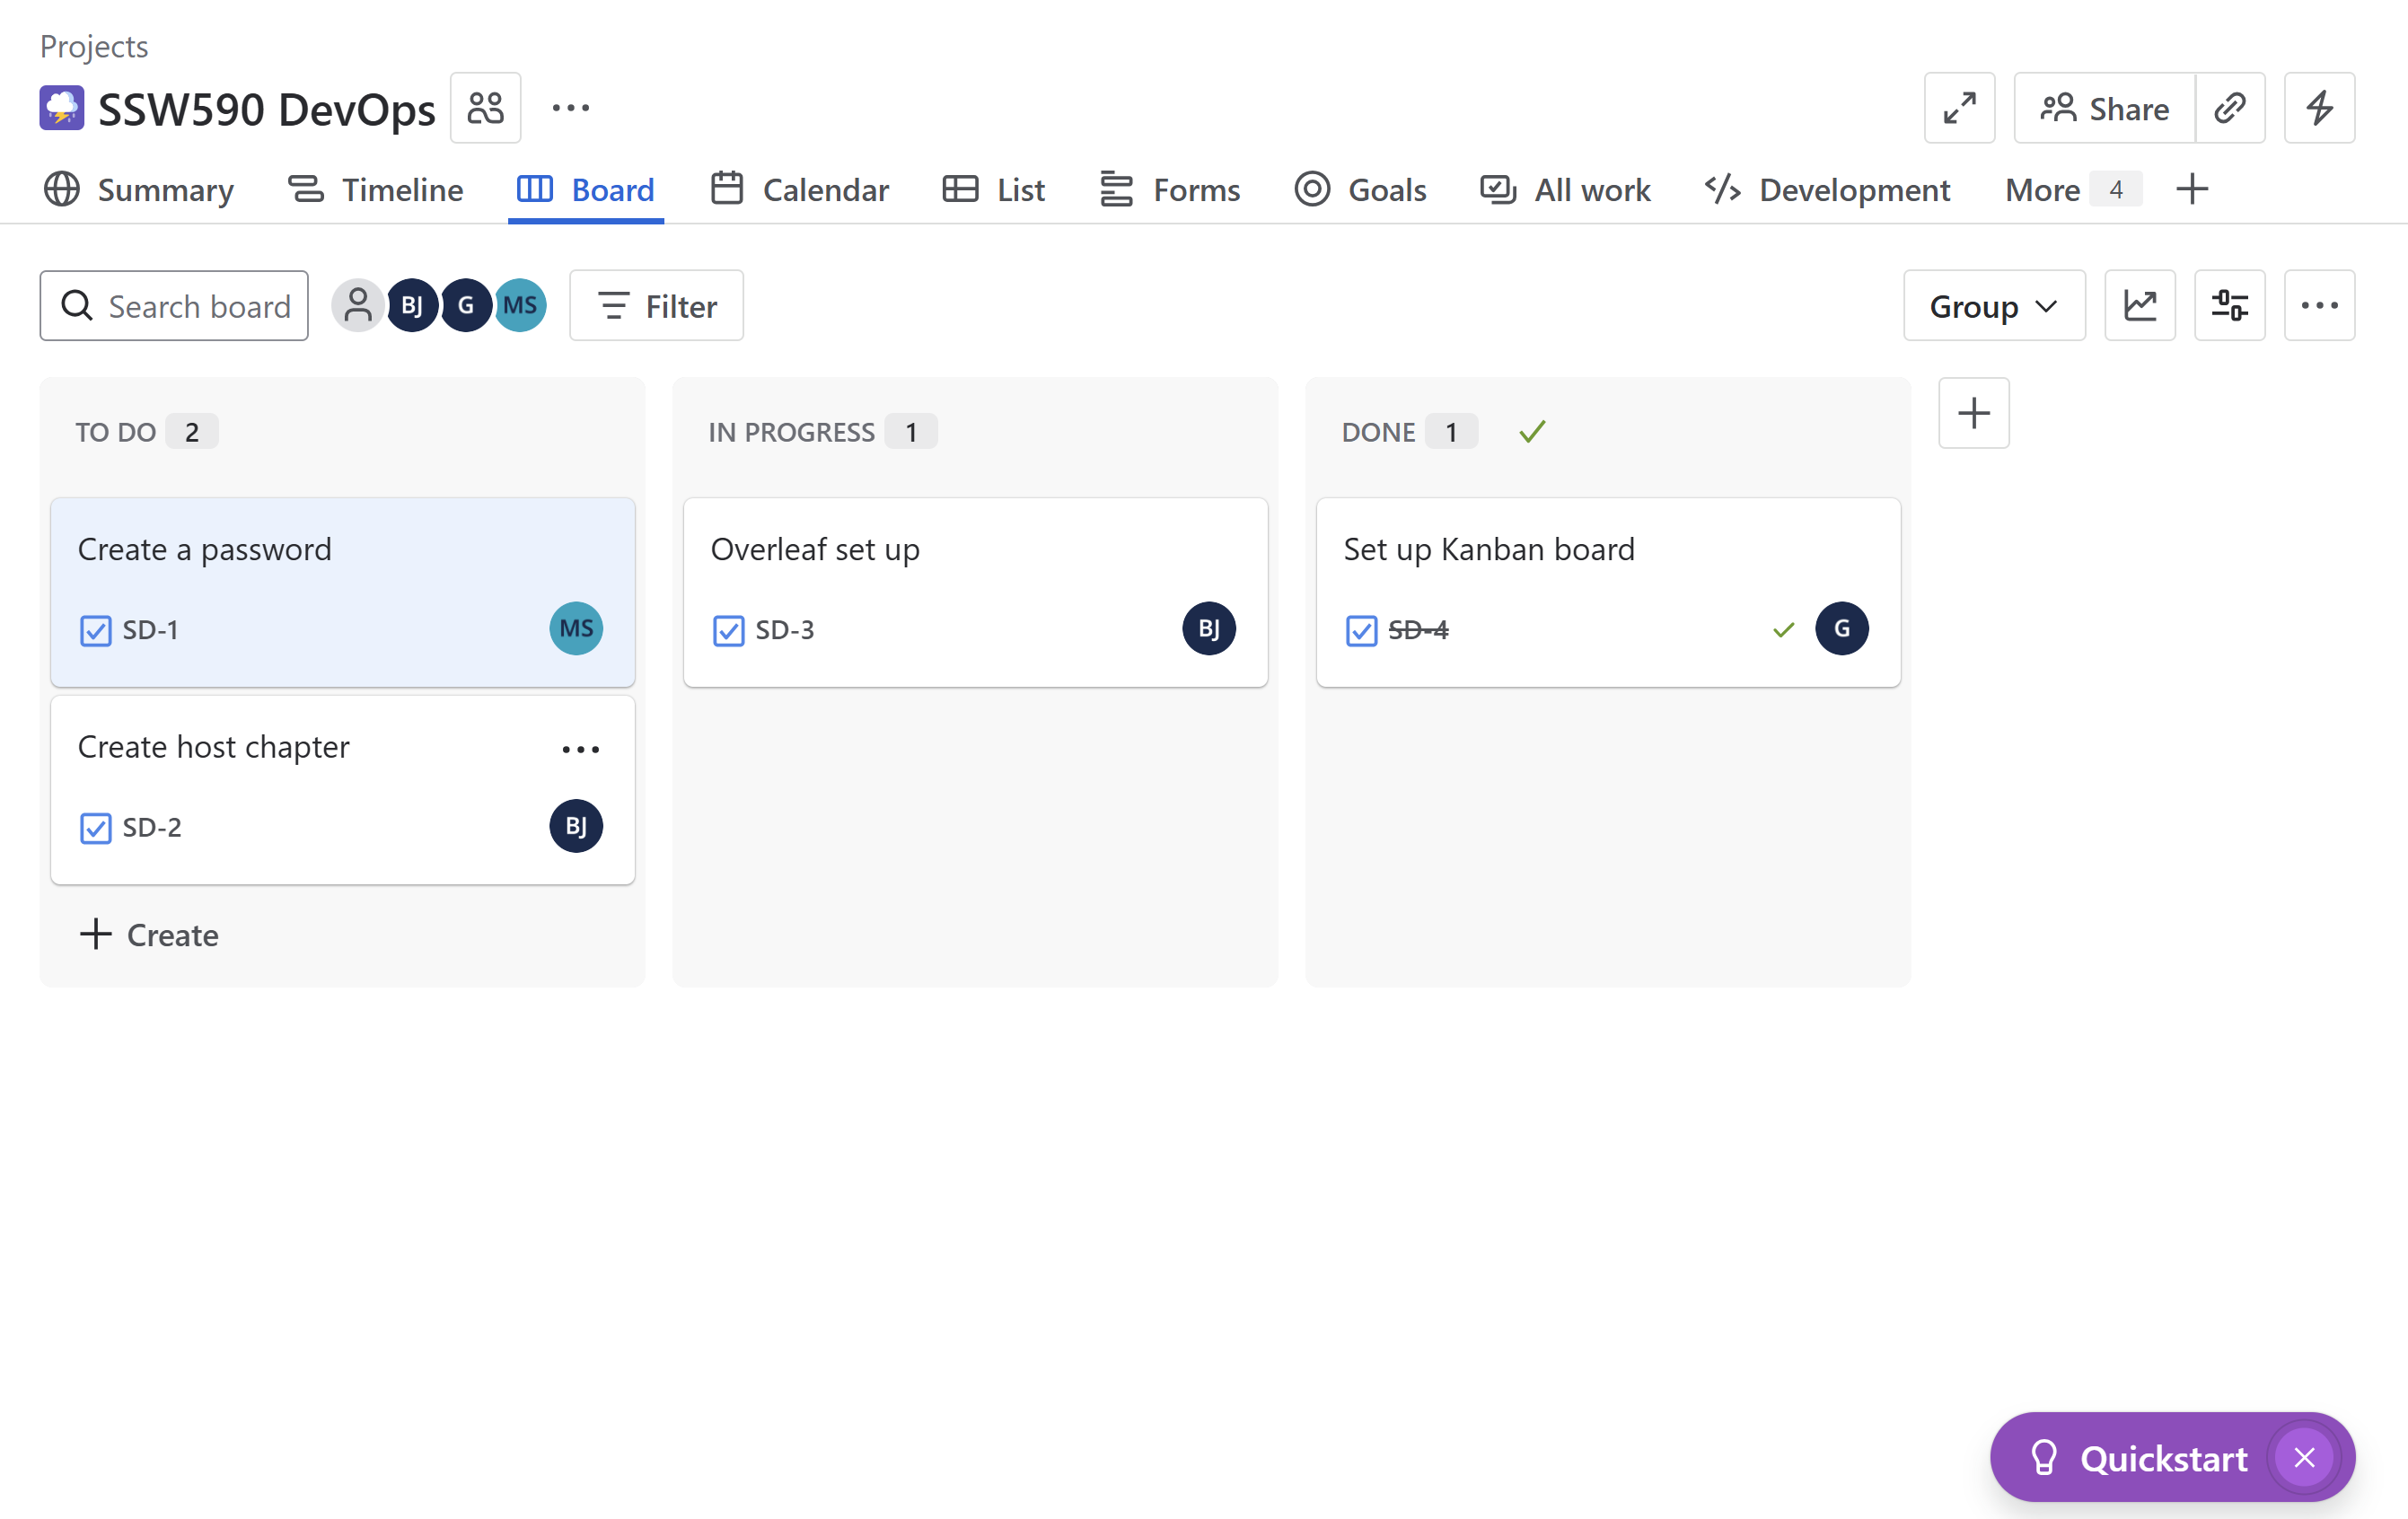
\includegraphics[width=\textwidth]{Kanban Board.png}
  \centering
  \caption{Kanban Board}
  \vspace{-0.3cm}
\end{figure}


\newpage
To organize the DevOps tasks, we created a Kanban board in \textbf{Atlassian Jira}

\section{Steps to Set Up the Kanban Board}

\begin{enumerate}
    \item \textbf{Create a Project in Jira} \\
    Logged into Jira and selected \textit{Create Project}. 
    Chose the \textit{Kanban template},
    Named the project \textbf{SSW590 DevOps}. Then share the Jira project with other teammates. 

    \item \textbf{Add Tasks (Issues)} \\
    Created individual issues for each assignment requirement:
    \begin{itemize}
        \item SD-1: Create a password
        \item SD-2: Create host chapter
        \item SD-3: Overleaf set up
        \item SD-4: Set up Kanban board
    \end{itemize}
    Tasks are assigned to each team member to ensure the workload for each team member is roughly the same.

    \item \textbf{Move Tasks Through Workflow} \\
    Dragged issues into the appropriate columns as progress was made:
    \begin{itemize}
        \item SD-4: Set up Kanban board $\rightarrow$ \textbf{Done}
        \item SD-3: Overleaf set up $\rightarrow$ \textbf{In Progress}
        \item SD-1: Create a password $\rightarrow$ \textbf{To Do}
        \item SD-2: Create host chapter $\rightarrow$ \textbf{To Do}
    \end{itemize}

    \item \textbf{Track Ownership and Progress} \\
    Each issue was labeled with an assignee.
    The board provides a clear snapshot of progress, bottlenecks, and remaining work.

\end{enumerate}